
%%%%%%%%%%%%%%%%%%%%%%%%%%%%%%%%%%%%%%%%%%%%%%%%%%%%%%%%%%%%%%%%%%%%%%%%%%%%%%
%                                                                            %
%  ************************** AVISO IMPORTANTE **************************    %
%                                                                            %
% Éste es un documento de ayuda para los autores que deseen enviar           %
% trabajos para su consideración en el Boletín de la Asociación Argentina    %
% de Astronomía.                                                             %
%                                                                            %
% Los comentarios en este archivo contienen instrucciones sobre el formato   %
% obligatorio del mismo que complementan los instructivos web y PDF.         %
% Por favor léalos.                                                          %
%                                                                            %
% No deben borrarse los comentarios en este archivo. En caso contrario,      %
% el sistema de recepción de manuscritos no permitirá el envío de su         %
% contribución. No se permite el uso de \newcommand ni definiciones          %
% particulares de cada autor.                                                %
%                                                                            %
%%%%%%%%%%%%%%%%%%%%%%%%%%%%%%%%%%%%%%%%%%%%%%%%%%%%%%%%%%%%%%%%%%%%%%%%%%%%%%

%%%%%%%%%%%%%%%%%%%%%%%%%%%%%%%%%%%%%%%%%%%%%%%%%%%%%%%%%%%%%%%%%%%%%%%%%%%%%%
%                                                                            %
%  ************************** IMPORTANT NOTICE **************************    %
%                                                                            %
%  This is a help file for authors who are preparing manuscripts to be       %
%  considered for publication in the Boletín de la Asociación Argentina      %
%  de Astronomía.                                                            %
%                                                                            %
%  The comments in this file give instructions about the manuscripts'        %
%  mandatory format that complement the instructions distributed as a PDF    %
%  and findable in the BAAA web. Please read them.                           %
%                                                                            %
%  The comments in this file must not be deleted. Otherwise, your            %
%  contribution will be rejected by the manuscript reception system.         %
%  The use of \newcommand and author definitions are forbidden.              %
%                                                                            %
%%%%%%%%%%%%%%%%%%%%%%%%%%%%%%%%%%%%%%%%%%%%%%%%%%%%%%%%%%%%%%%%%%%%%%%%%%%%%%

\documentclass[baaa]{baaa}

\usepackage[pdftex]{hyperref}
\usepackage{subfigure}
\usepackage{natbib}
\usepackage{helvet,soul}
\usepackage[font=small]{caption}

%%%%%%%%%%%%%%%%%%%%%%%%%%%%%%%%%%%%%%%%%%%%%%%%%%%%%%%%%%%%%%%%%%%%%%%%%%%%%%
%                                                                            %
%  Seleccione el idioma de su contribución: Recuerde que todos los           %
%  componentes del documento (titulo, texto, figuras, tablas, etc.)          %
%  deben estar en el mismo idioma.                                           %
%                                                                            %
%  Select the language of your contribution: Please remember that all       %
%  document parts (title, text, figures, tables, etc.) must be in the        %
%  same language.                                                            %
%                                                                            %
%  0: Castellano / Spanish                                                   %
%  1: Inglés / English                                                       %
%                                                                            %
%%%%%%%%%%%%%%%%%%%%%%%%%%%%%%%%%%%%%%%%%%%%%%%%%%%%%%%%%%%%%%%%%%%%%%%%%%%%%%

\contriblanguage{0}

%%%%%%%%%%%%%%%%%%%%%%%%%%%%%%%%%%%%%%%%%%%%%%%%%%%%%%%%%%%%%%%%%%%%%%%%%%%%%%
%                                                                            %
%  Seleccione el tipo de contribución solicitada:                            %
%                                                                            %
%  Select the requested contribution type:                                   %
%                                                                            %
%  1: Presentación mural / Poster                                            %
%  2: Presentación oral / Oral contribution                                  %
%  3: Informe invitado / Invited report                                      %
%  4: Mesa redonda / Round table                                             %
%  5: Presentación Premio Varsavsky / Varsavsky Prize contribution           %
%  6: Presentación Premio Sahade / Sahade Prize contribution                 %
%  7: Presentación Premio Sérsic / Sérsic Prize contribution                 %
%                                                                            %
%%%%%%%%%%%%%%%%%%%%%%%%%%%%%%%%%%%%%%%%%%%%%%%%%%%%%%%%%%%%%%%%%%%%%%%%%%%%%%

\contribtype{2}

%%%%%%%%%%%%%%%%%%%%%%%%%%%%%%%%%%%%%%%%%%%%%%%%%%%%%%%%%%%%%%%%%%%%%%%%%%%%%%
%                                                                            %
%  Seleccione el área temática de su contribución:                           %
%                                                                            %
%  Select the thematic area of your contribution:                            %
%                                                                            %
%  1 [AEC]:   Astrofísica Extragaláctica y Cosmología /                      %
%             Extragalactic Astrophysics and Cosmology                       %
%  2 [EG]:    Estructura Galáctica / Galactic Structure                      %
%  3 [AE]:    Astrofísica Estelar / Stellar Astrophysics                     %
%  4 [SE]:    Sistemas Estelares / Stellar Systems                           %
%  5 [ICSA]:  Instrumentación y Caracterización de Sitios Astronómicos /     %
%             Instrumentation and Astronomical Site Characterization         %
%  6 [MI]:    Medio Interestelar / Interstellar Medium                       %
%  7 [OCPAE]: Objetos Compactos y Procesos de Altas Energías /               %
%             Compact Objetcs and High-Energy Processes                      %
%  8 [SH]:    Sol y Heliosfera / Sun and Heliosphere                         %
%  9 [SSE]:   Sistemas Solar y Extrasolares / Solar and Extrasolar Systems   %
% 10 [HEDA]:  Historia, Enseñanza y Divulgación de la Astronomía /           %
%             History, Teaching and Spreading of Astronomy                   %
% 11 [O]:     Otros / Other Topics                                           %
%                                                                            %
%%%%%%%%%%%%%%%%%%%%%%%%%%%%%%%%%%%%%%%%%%%%%%%%%%%%%%%%%%%%%%%%%%%%%%%%%%%%%%

\thematicarea{8}

\title{Estudio de Validación Tomográfica del modelo MHD AWSoM}
%\subtitle{Instrucciones de estilo}

%%%%%%%%%%%%%%%%%%%%%%%%%%%%%%%%%%%%%%%%%%%%%%%%%%%%%%%%%%%%%%%%%%%%%%%%%%%%%%
%                                                                            %
%  Agregue un título corto para el encabezado de las páginas pares.          %
%                                                                            %
%  Add a short title to appear in the header of even pages.                  %
%                                                                            %
%%%%%%%%%%%%%%%%%%%%%%%%%%%%%%%%%%%%%%%%%%%%%%%%%%%%%%%%%%%%%%%%%%%%%%%%%%%%%%

\titlerunning{Macro BAAA61B con instrucciones de estilo}

%%%%%%%%%%%%%%%%%%%%%%%%%%%%%%%%%%%%%%%%%%%%%%%%%%%%%%%%%%%%%%%%%%%%%%%%%%%%%%
%                                                                            %
%  Lista de autores. Los nombres de los autores deben estar separados por    %
%  comas, y deben tener el formato A.E. Autor (iniciales apellido(s); sin    %
%  coma entre apellido e iniciales ni espacios entre las iniciales).         %
%                                                                            %
%  Author list. Authors' names must be separated by commas, and stick to     %
%  the format A.E. Author (initials Family name -neither commas between      %
%  name and the initials nor blanks between the initials).                   %
%                                                                            %
%%%%%%%%%%%%%%%%%%%%%%%%%%%%%%%%%%%%%%%%%%%%%%%%%%%%%%%%%%%%%%%%%%%%%%%%%%%%%%

\author{D.G. Lloveras\inst{1}, A.M. Vásquez\inst{1}, F.A. Nuevo\inst{1}, C. Mac Cormack\inst{1}, N. Sachdeva\inst{2},\\ W. Manchester IV\inst{2}, B. Van der Holst\inst{2}, \& R.A. Frazin\inst{2}}
\authorrunning{Lloveras et al.}


%%%%%%%%%%%%%%%%%%%%%%%%%%%%%%%%%%%%%%%%%%%%%%%%%%%%%%%%%%%%%%%%%%%%%%%%%%%%%%
%                                                                            %
% Por favor provea una dirección de e-mail de contacto para los lectores.    %
%                                                                            %
% Please provide a contact e-mail address for the readers.                   %
%                                                                            %
%%%%%%%%%%%%%%%%%%%%%%%%%%%%%%%%%%%%%%%%%%%%%%%%%%%%%%%%%%%%%%%%%%%%%%%%%%%%%%

\contact{dlloveras@iafe.uba.ar}

\institute{
Insituto de Astronomía y Física del Espacio, CONICET--UBA, Argentina \and
Climate and Space Sciences and Engineering, Universidad de Michigan, EEUU.
}

%%%%%%%%%%%%%%%%%%%%%%%%%%%%%%%%%%%%%%%%%%%%%%%%%%%%%%%%%%%%%%%%%%%%%%%%%%%%%%
%                                                                            %
%  El resumen y el abstract son ambos obligatorios, independientemente del   %
%  lenguaje elegido.                                                         %
%                                                                            %
%  The Resumen and the abstract are both mandatory, regardless of the chosen %
%  language.                                                                 %
%                                                                            %
%%%%%%%%%%%%%%%%%%%%%%%%%%%%%%%%%%%%%%%%%%%%%%%%%%%%%%%%%%%%%%%%%%%%%%%%%%%%%%

\resumen{
Los modelos magnetohidrodinámicos (MHD) tridimensionales (3D),  necesarios para modelar y predecir el clima espacial, deben ser validados observacionalmente. A escala global, esto puede ser hecho mediante tomografía de medida de emisión diferencial (DEMT), que provee resultados 3D de densidad y temperatura electrónica en la baja corona ($1.0-1.25 \, \rm{R}_\odot$). Realizamos una validación DEMT de la versión mas reciente del Alfvén Wave Solar Model (AWSoM) del Space Weather Modeling Framework (SWMF). Se lleva a cabo un análisis comparativo a lo largo de las líneas de campo de la densidad y temperatura electrónicas del modelo y la tomografía, así como de cantidades energéticas integrales. Para este estudio se seleccionaron dos rotaciones de mínimo solar, una entre los ciclos solares (SC) 23 y 24, y otra entre los SCs 24 y 25. Discutimos las diferencias observadas entre el modelo y los productos tomográficos, y las limitaciones y posibles mejoras futuras para el modelo AWSoM.)
}

%Discutimos las diferencias observadas ente el modelo y los productos tomográficos, y las limitaciones y posibles mejoras futuras para el modelo AWSoM (no me deja poner mas lineas!)
\abstract{
Aiming model and forecast the space climate, the tri-dimensional (3D) magnetohydrodinamic (MHD) models are in need of observational validations. This can be done using the differential emission measure technique (DEMT) which provides 3D results of electronic density and temperature in the low corona ($1.0-1.25 \, \rm{R}_\odot$). We performed a DEMT validation of the last version of the Alfvén Wave Solar Model (AWSoM) within the Space Weather Modeling Framework (SWMF). We carried out a comparative analysis along de magnetic field lines using thermodynamic quantities of the model and the tomography results. In this study we selected two rotations othe solar minimum between solar cicle (SC) 23 and 24, and the other one between SCs 24 and 25. We discuss the difference observed between the model and the observations, the limitations and the possible upgrades to the AWSOM model.)
}

%%%%%%%%%%%%%%%%%%%%%%%%%%%%%%%%%%%%%%%%%%%%%%%%%%%%%%%%%%%%%%%%%%%%%%%%%%%%%%
%                                                                            %
%  Seleccione las palabras clave que describen su contribución. Las mismas   %
%  son obligatorias, y deben tomarse de la lista de la American Astronomical %
%  Society (AAS), que se encuentra en la página web indicada abajo.          %
%                                                                            %
%  Select the keywords that describe your contribution. They are mandatory,  %
%  and must be taken from the list of the American Astronomical Society      %
%  (AAS), which is available at the webpage quoted below.                    %
%                                                                            %
%  https://aas.org/authors/astronomical-subject-keywords-update-august-2013  %
%                                                                            %
%%%%%%%%%%%%%%%%%%%%%%%%%%%%%%%%%%%%%%%%%%%%%%%%%%%%%%%%%%%%%%%%%%%%%%%%%%%%%%

\keywords{Sun: corona — Sun: fundamental parameters — Sun: UV radiation — Sun: abundances}

\begin{document}

\maketitle

\section{Introducción}
\label{S_intro}


\section{Método}


\section{Resultados}



%%%%%%%%%%%%%%%%%%%%%%%%%%%%%%%%%%%%%%%%%%%%%%%%%%%%%%%%%%%%%%%%%%%%%%%%%%%%%%
%                                                                            %
% Para figuras de dos columnas use \begin{figure*} ... \end{figure*}         %
%                                                                            %
%%%%%%%%%%%%%%%%%%%%%%%%%%%%%%%%%%%%%%%%%%%%%%%%%%%%%%%%%%%%%%%%%%%%%%%%%%%%%%

\section{Discusion}


\section{Resultados}

\begin{figure*}
  \centering
  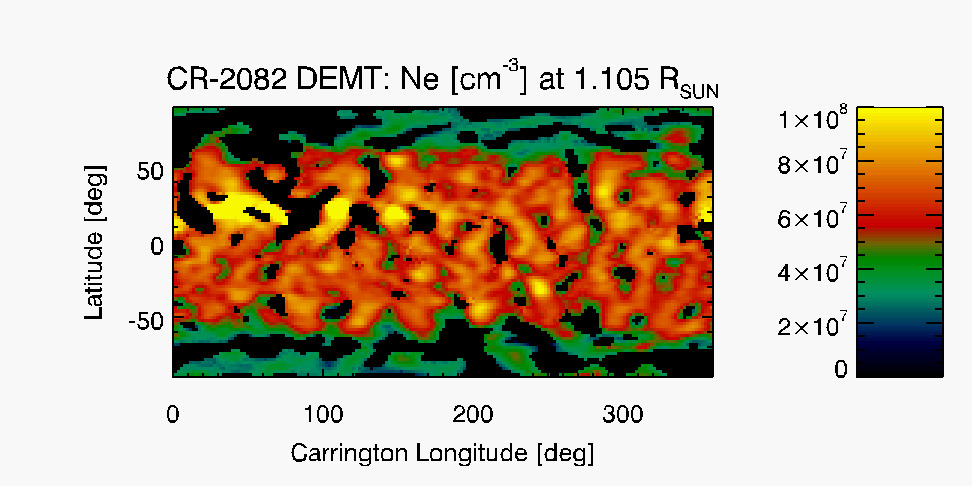
\includegraphics[width=0.4\textwidth]{figuras/map_Ne_CR2082_DEMT-EUVI_behind_H1-L3523_r3d_1105_Rsun.jpg}
  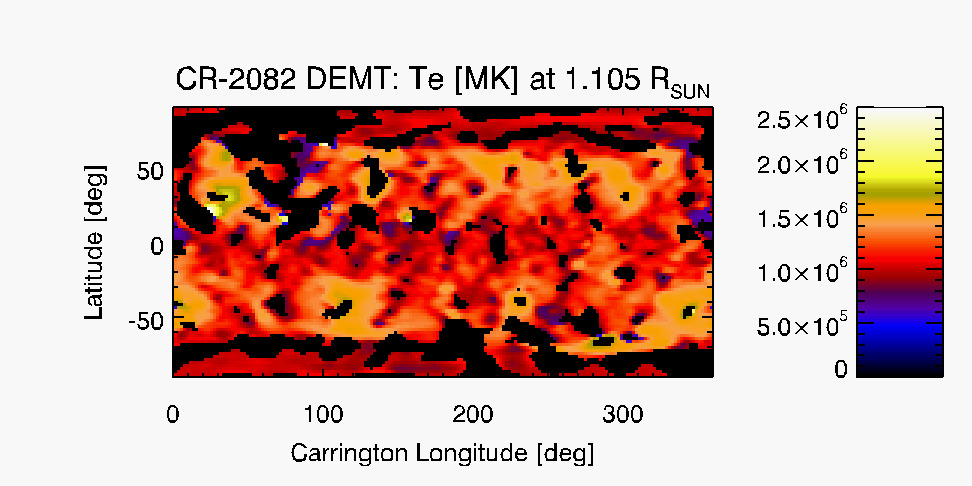
\includegraphics[width=0.4\textwidth]{figuras/map_Tm_CR2082_DEMT-EUVI_behind_H1-L3523_r3d_1105_Rsun.jpg}
  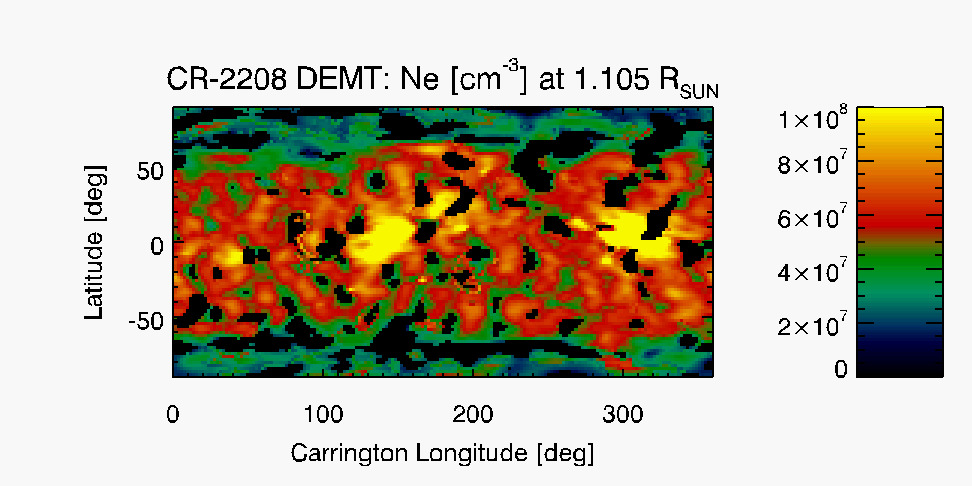
\includegraphics[width=0.4\textwidth]{figuras/map_Ne_CR2208_DEMT-AIA_H1_L522_r3d_1105_Rsun.jpg}
  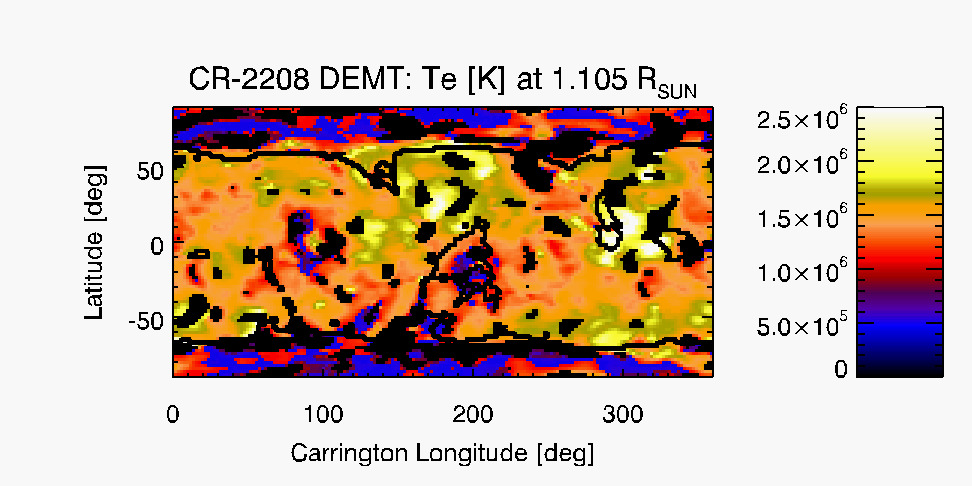
\includegraphics[width=0.4\textwidth]{figuras/map_Tm_CR2208_DEMT-AIA_H1_L522_r3d_1105_Rsun.jpg}
  \caption{Mapas de Carrington de densidad y temperatura electrónica de CR-2082 y CR-2208 de resultados tomográficos en la altura  1.105 ${\rm R_\odot}$.}
  \label{fig-carrington1}
\end{figure*}
  \begin{figure*}
  \centering
  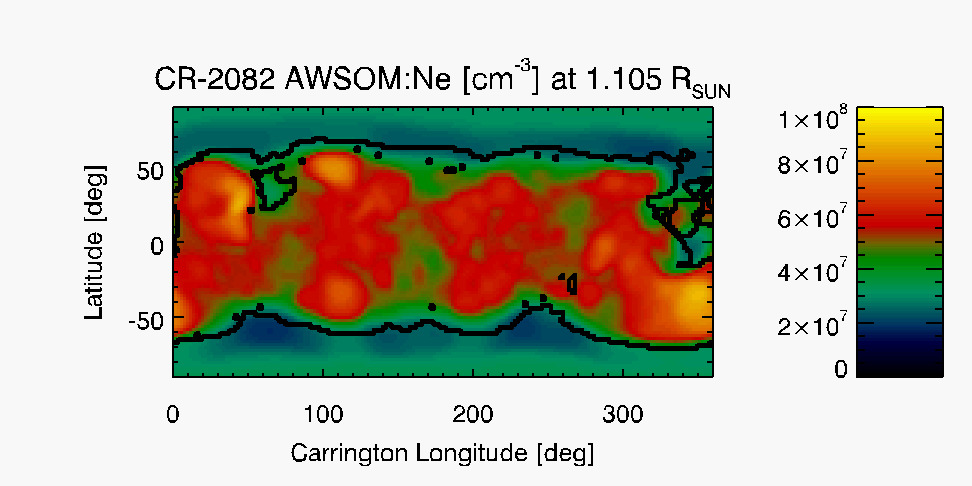
\includegraphics[width=0.4\textwidth]{figuras/map_Ne_awsom_2082_185_short_1105_Rsun.jpg}
  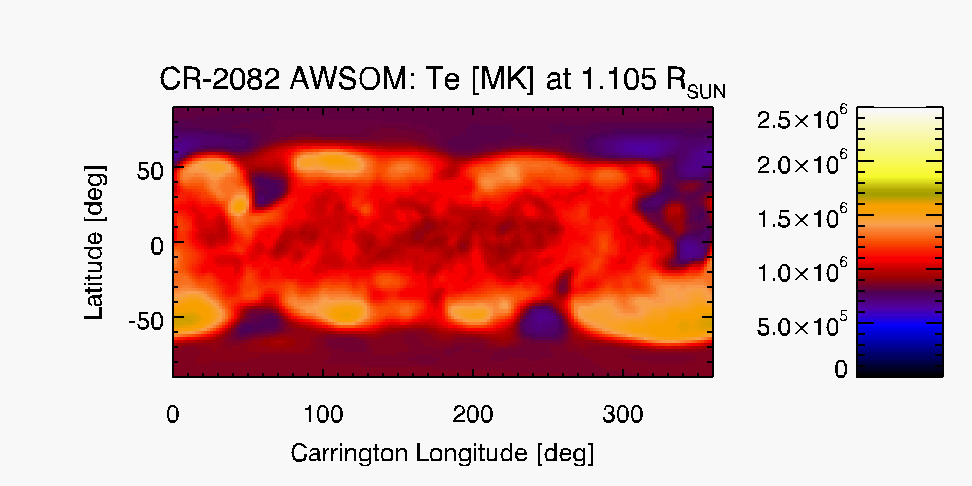
\includegraphics[width=0.4\textwidth]{figuras/map_Te_awsom_2082_185_short_1105_Rsun.jpg}
  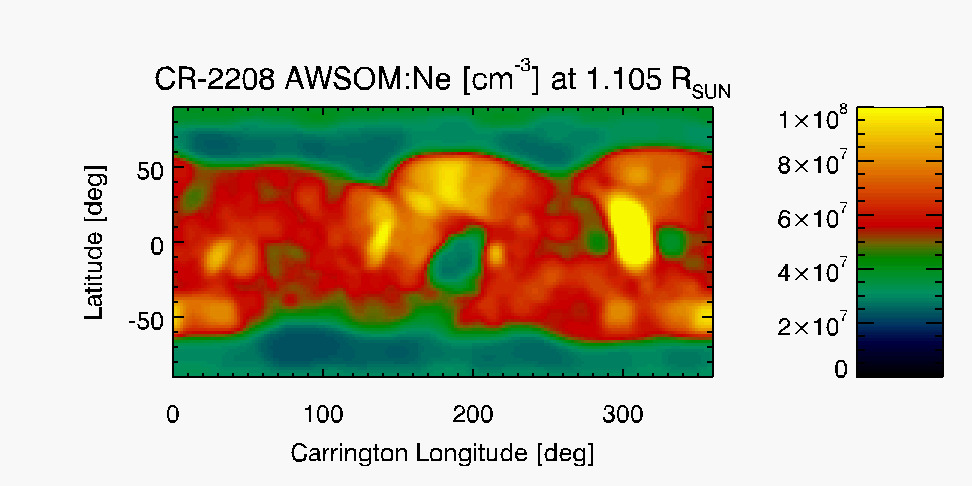
\includegraphics[width=0.4\textwidth]{figuras/map_Ne_awsom_2208_185_1105_Rsun.jpg}
  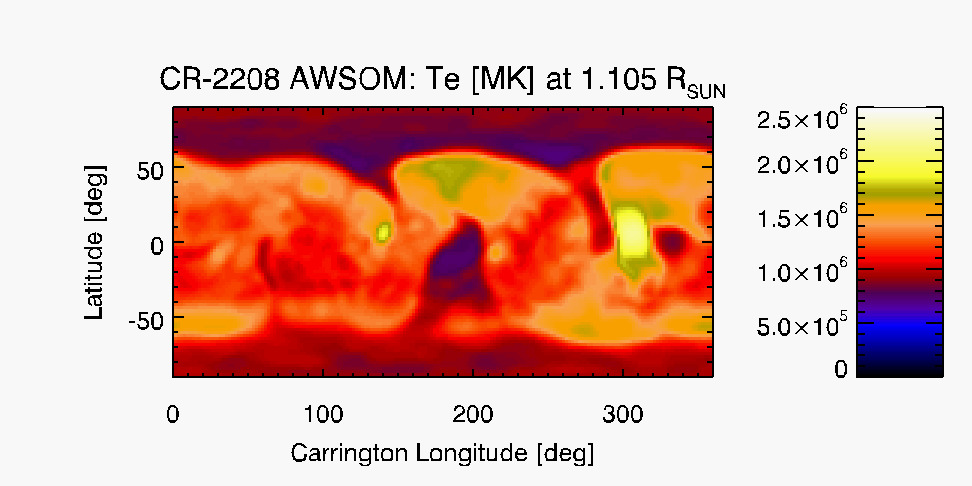
\includegraphics[width=0.4\textwidth]{figuras/map_Te_awsom_2208_185_1105_Rsun.jpg}
  \caption{Igual que figura \ref{fig-carrington1} pero para resultados del modelo AWSOM.}
  \label{fig-carrington2}
\end{figure*}


\begin{figure*}
  \centering
  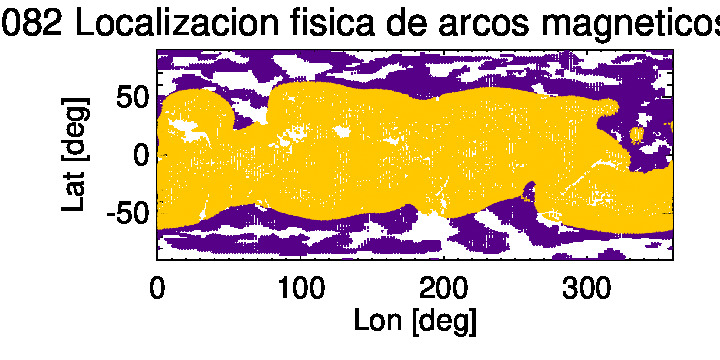
\includegraphics[width=0.4\textwidth]{figuras/proceeding2019_1105_2082_demt_Rpoint-map.jpg}
  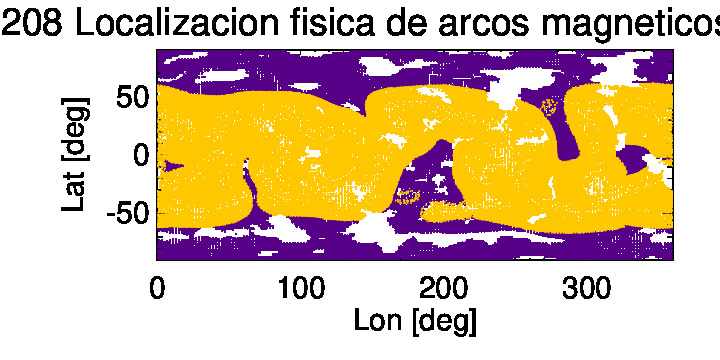
\includegraphics[width=0.4\textwidth]{figuras/proceeding2019_1105_2208_demt_Rpoint-map.jpg}
  \caption{Lolcalización física d elos arcos magnéticos a 1.105 ${\rm R_\odot}$. En amarillo la región cerrada y en violeta la región abierta.}
  \label{fig-rpoint}
\end{figure*}

\begin{figure*}
  \centering
  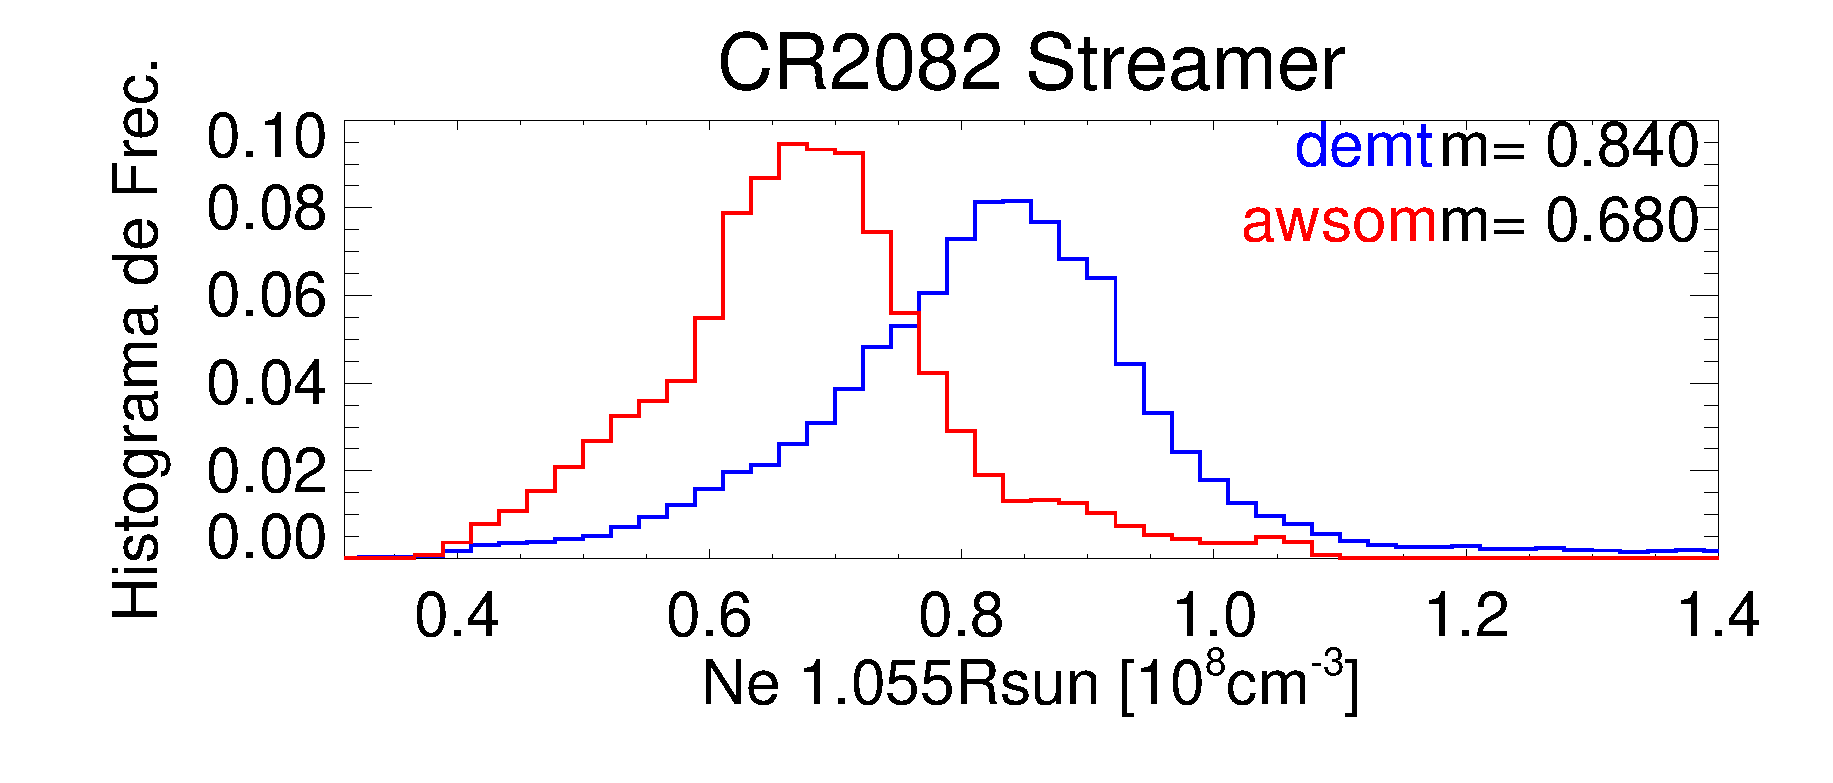
\includegraphics[width=0.32\textwidth]{figuras/proceeding_2082_demt_awsom_streamer_ne_1055.eps}
  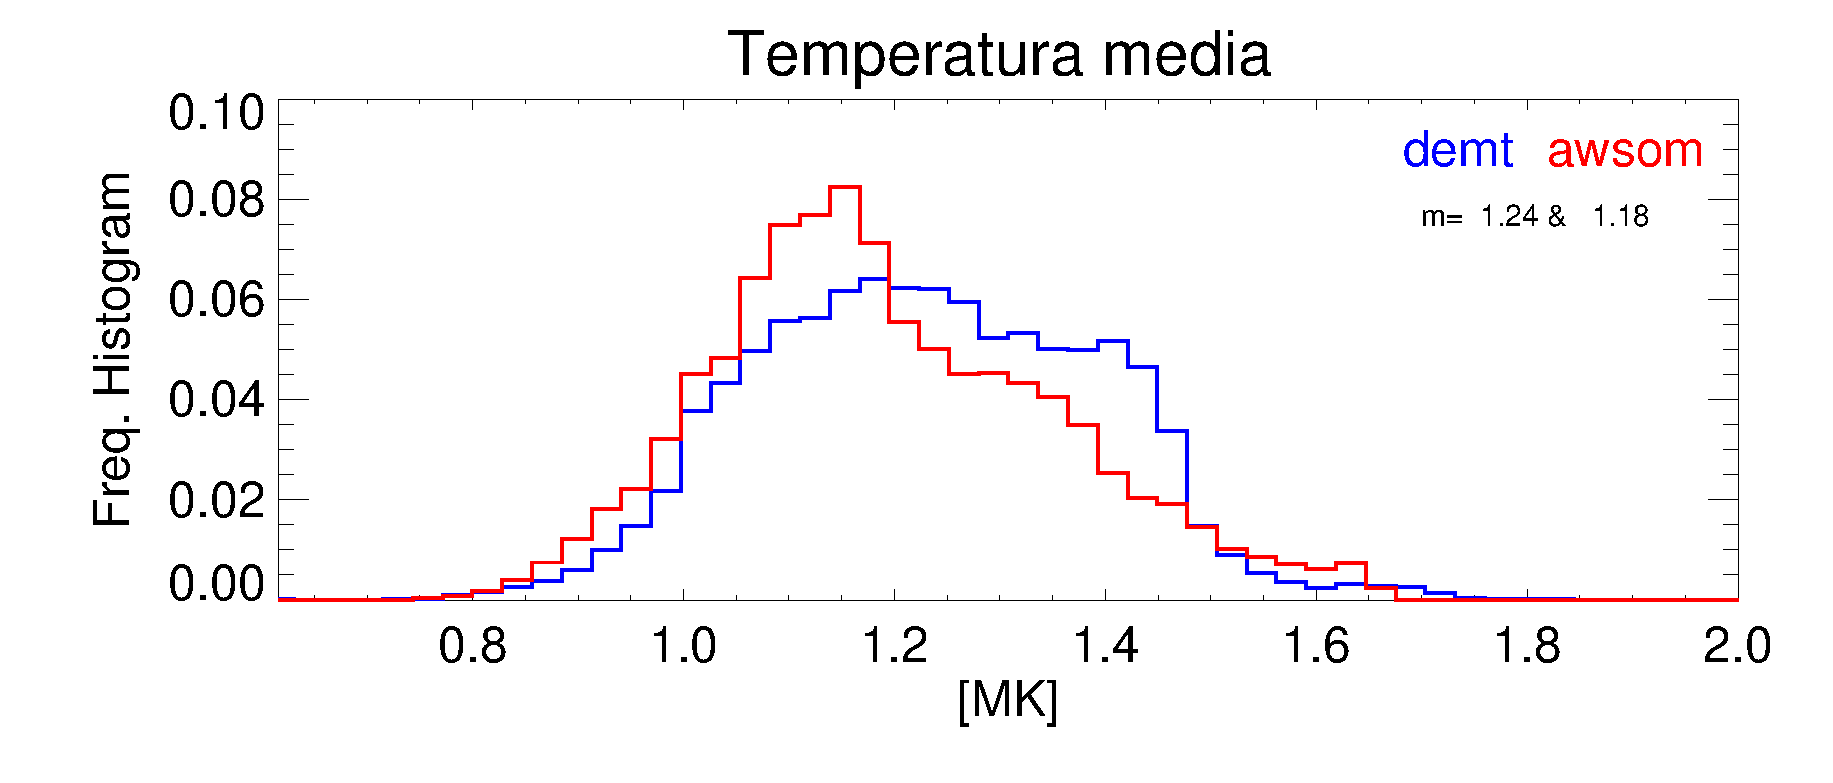
\includegraphics[width=0.32\textwidth]{figuras/proceeding_2082_demt_awsom_streamer_Tm.eps}
  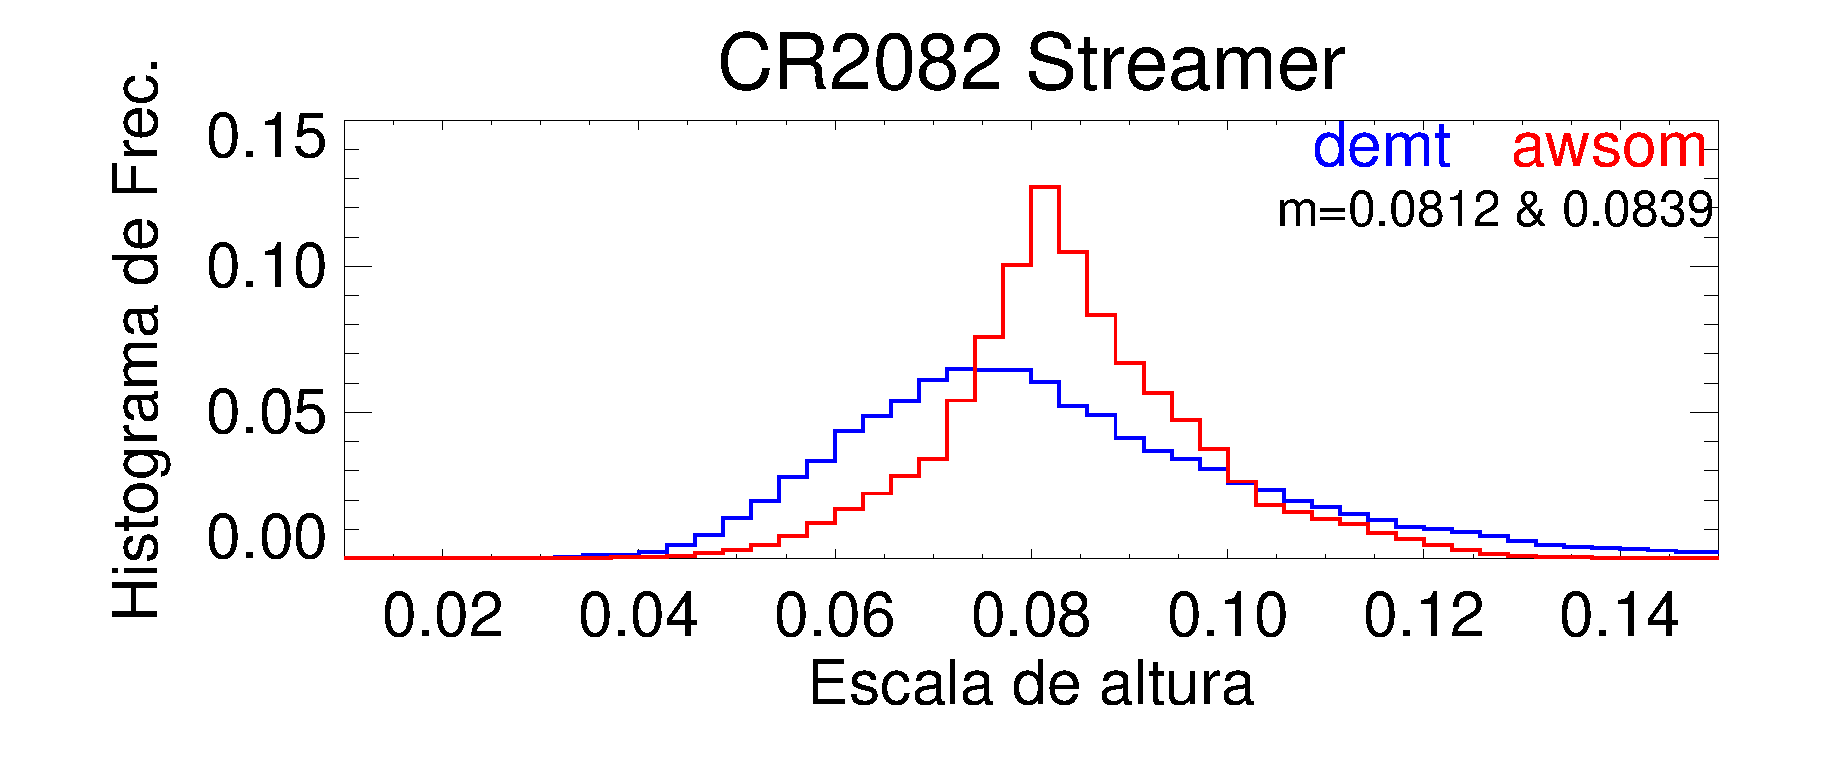
\includegraphics[width=0.32\textwidth]{figuras/proceeding_2082_demt_awsom_streamer_lambda_n.eps}\\
  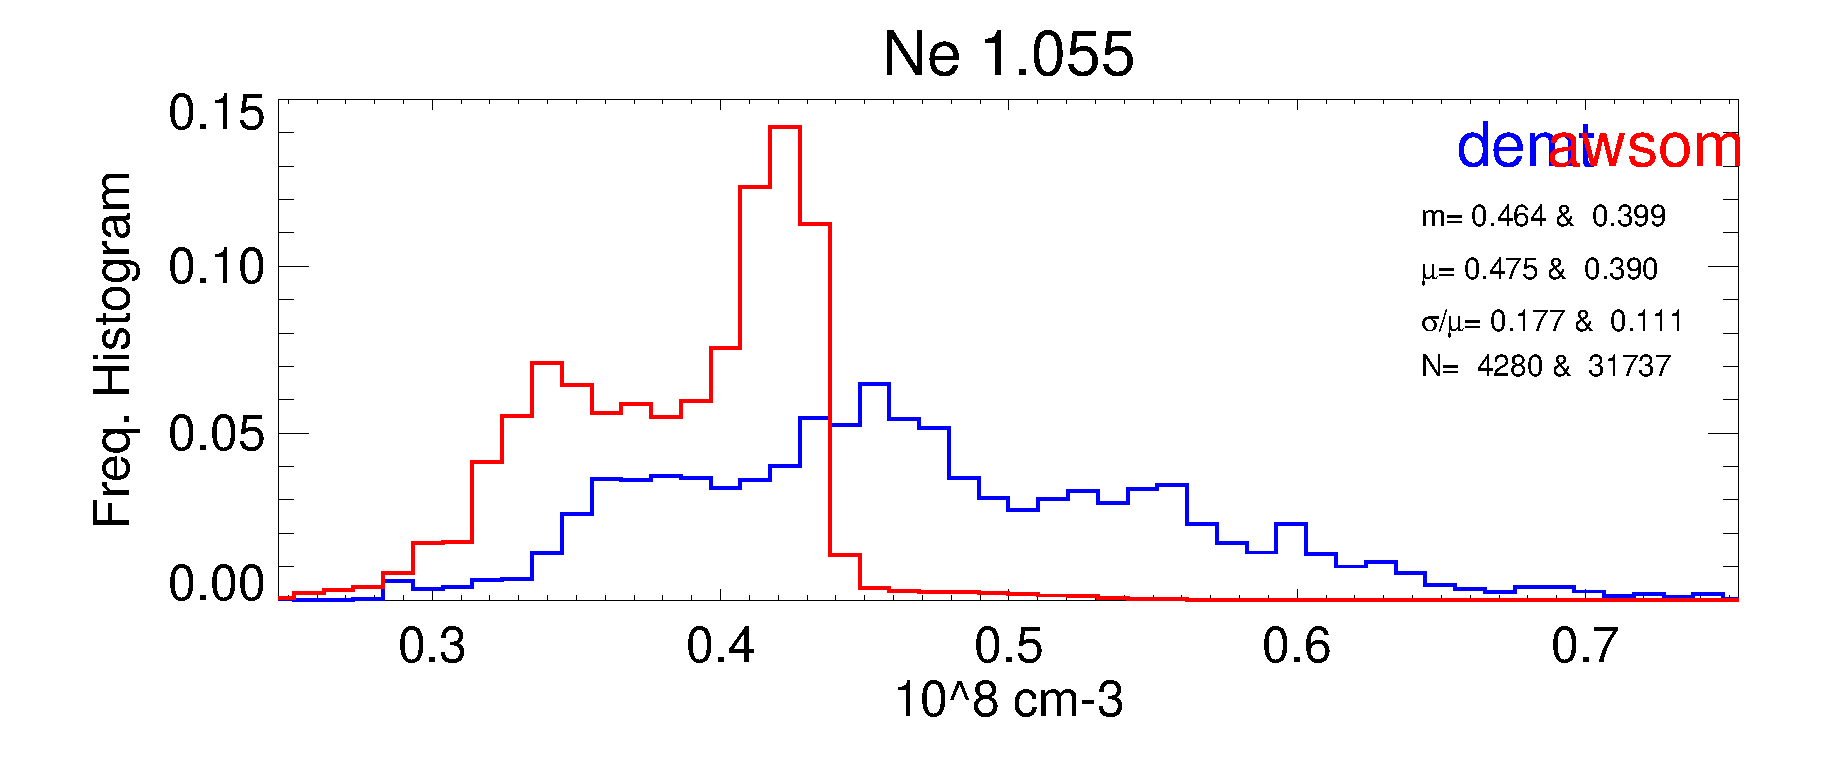
\includegraphics[width=0.32\textwidth]{figuras/proceeding_2082_demt_awsom_CH_ne_1055.eps}
  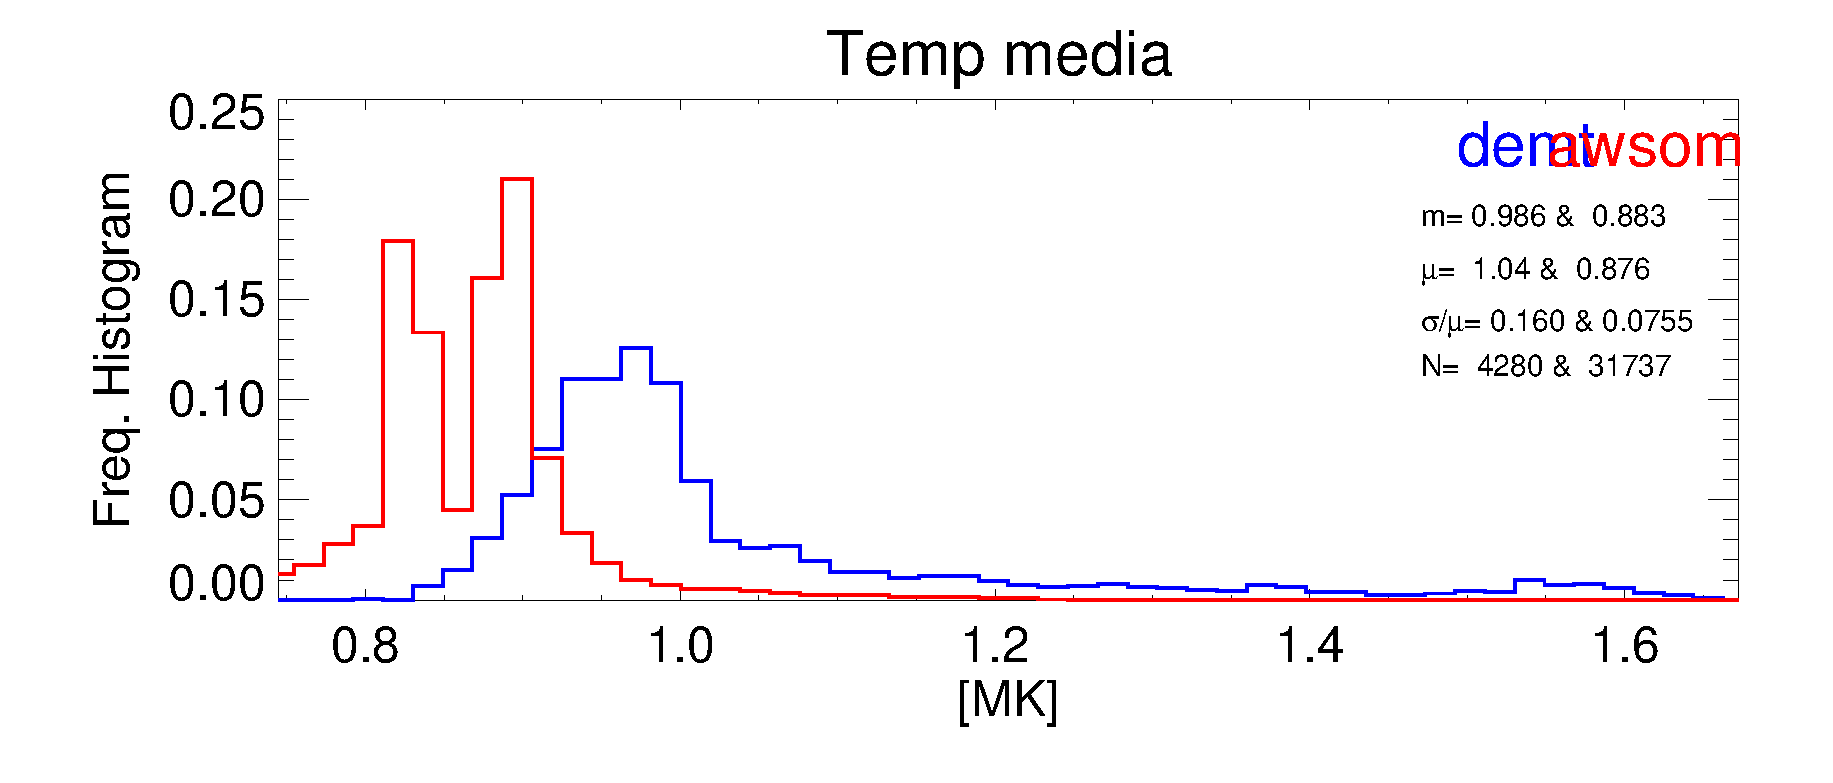
\includegraphics[width=0.32\textwidth]{figuras/proceeding_2082_demt_awsom_CH_Tm.eps}
  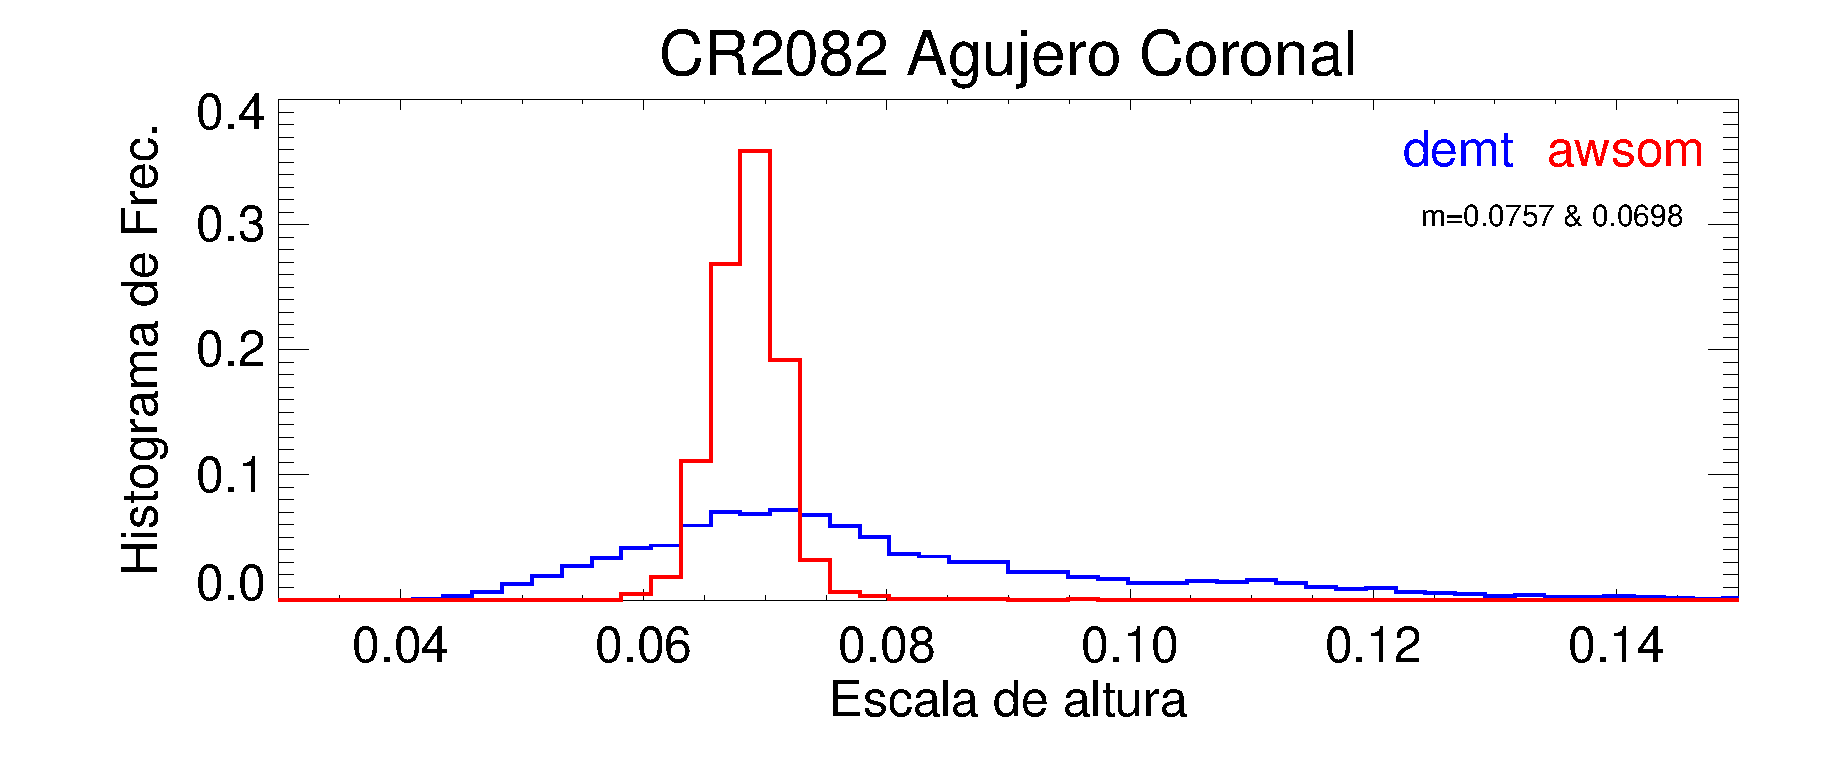
\includegraphics[width=0.32\textwidth]{figuras/proceeding_2082_demt_awsom_CH_lambda_n.eps}
  \caption{Histogramas}
  \label{fig-histos}
\end{figure*}

\begin{figure*}
  \centering
  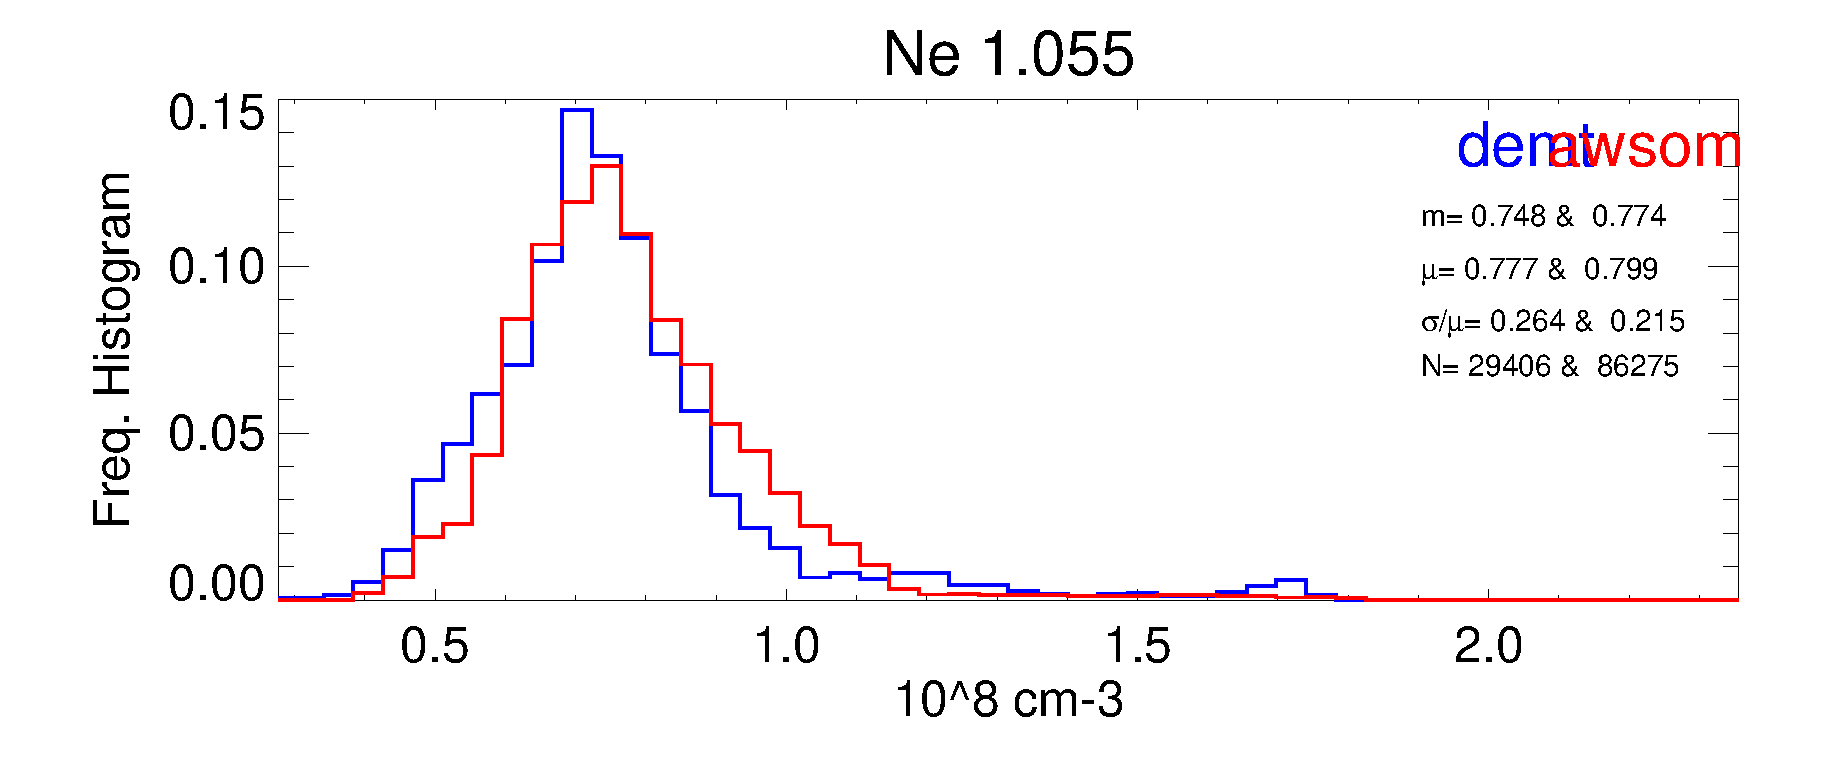
\includegraphics[width=0.32\textwidth]{figuras/proceeding_2208_demt_awsom_streamer_ne_1055.eps}
  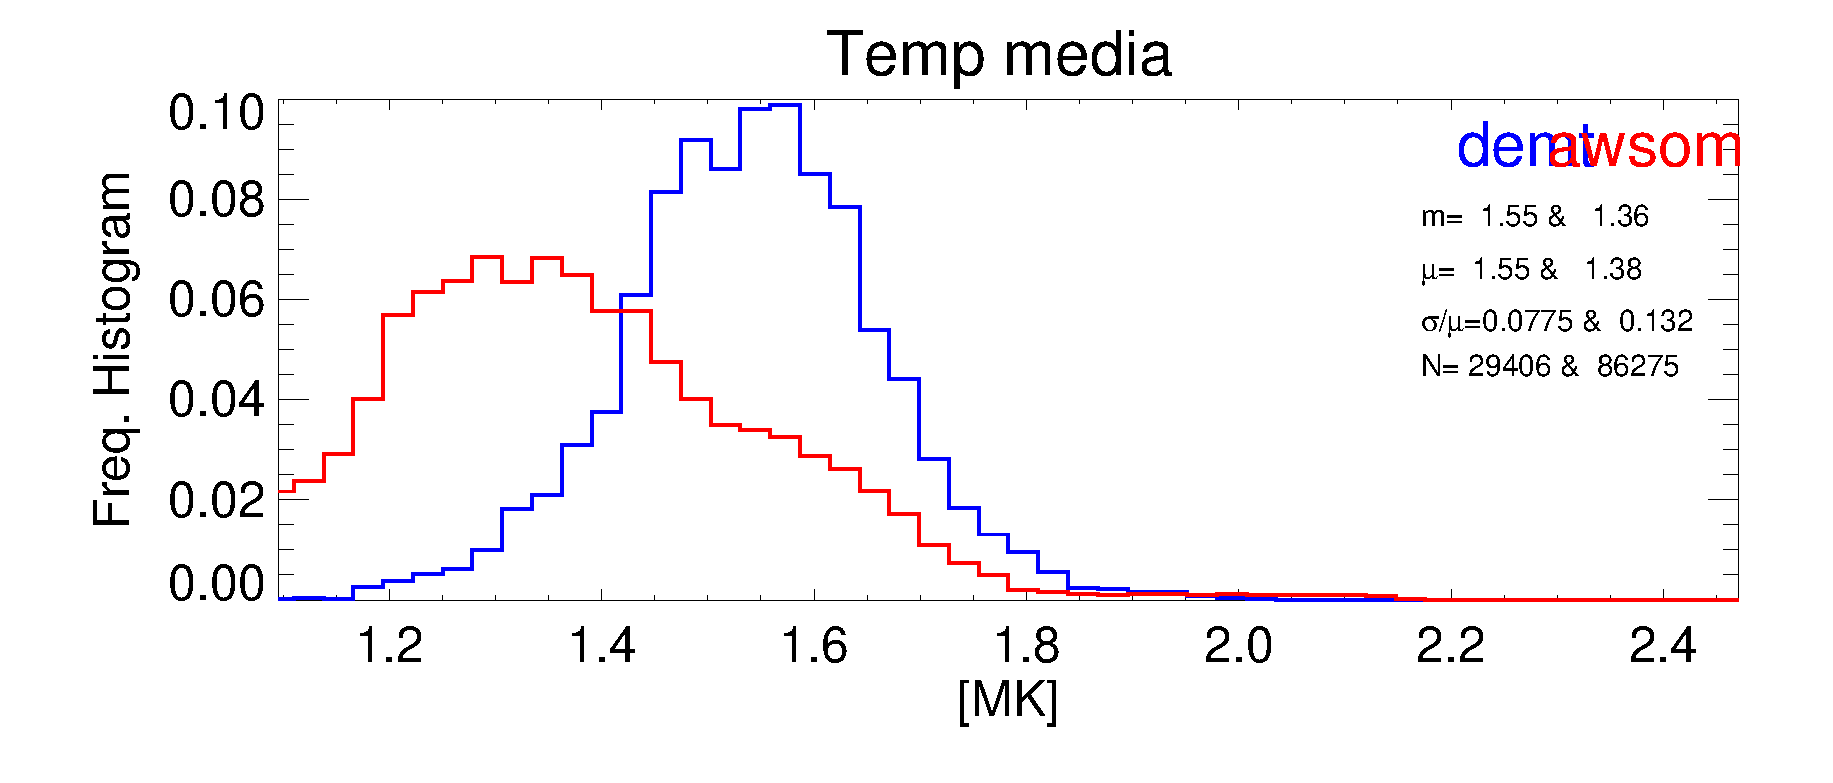
\includegraphics[width=0.32\textwidth]{figuras/proceeding_2208_demt_awsom_streamer_Tm.eps}
  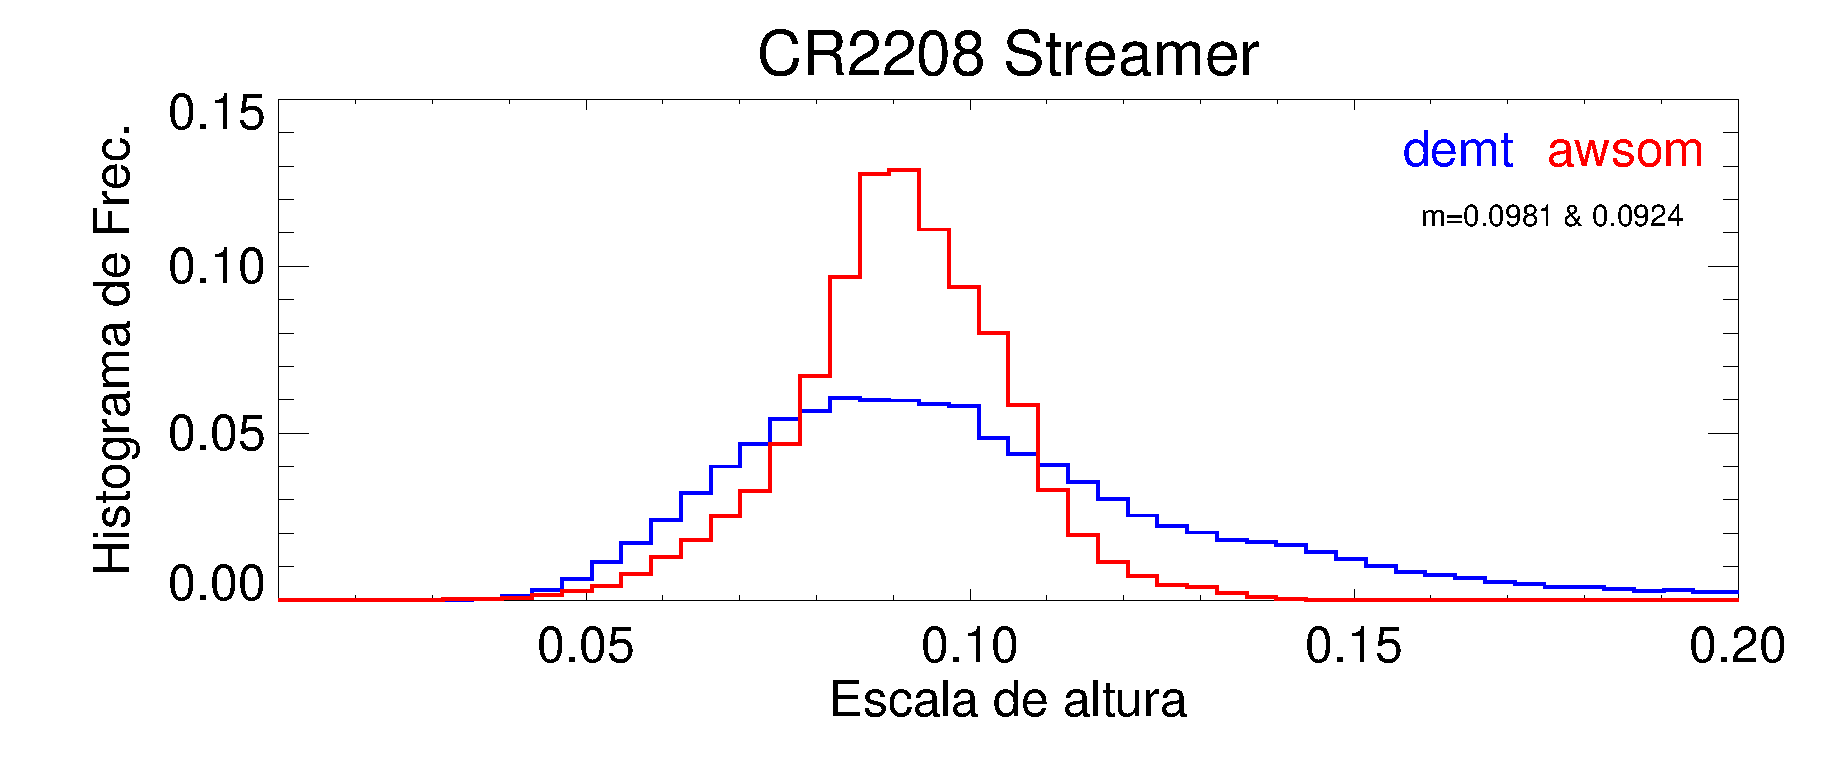
\includegraphics[width=0.32\textwidth]{figuras/proceeding_2208_demt_awsom_streamer_lambda_n.eps}\\
  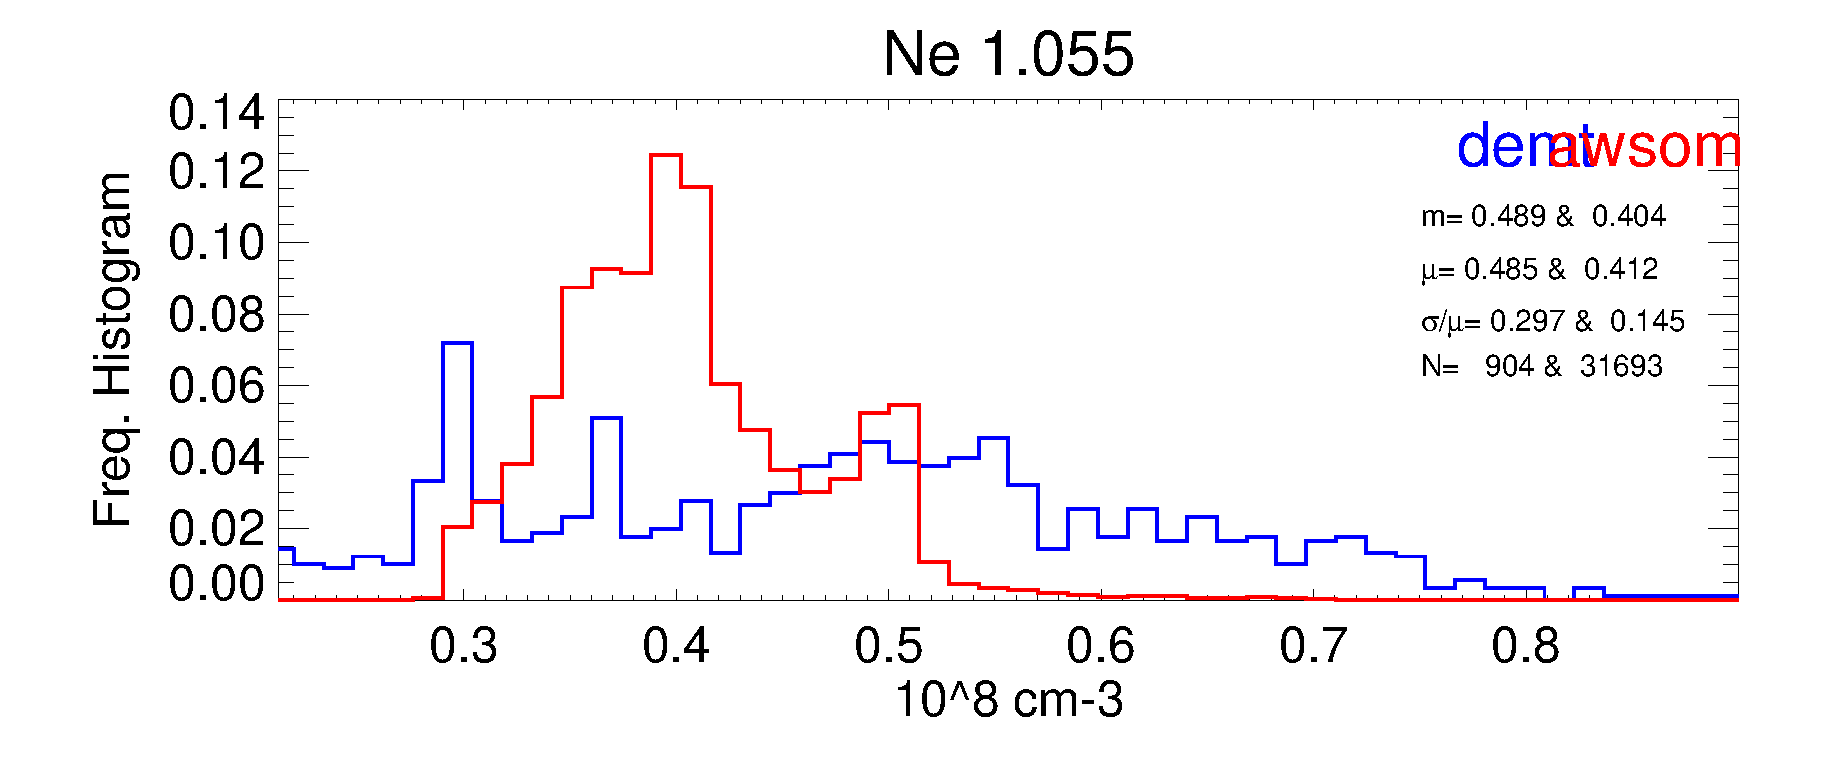
\includegraphics[width=0.32\textwidth]{figuras/proceeding_2208_demt_awsom_CH_ne_1055.eps}
  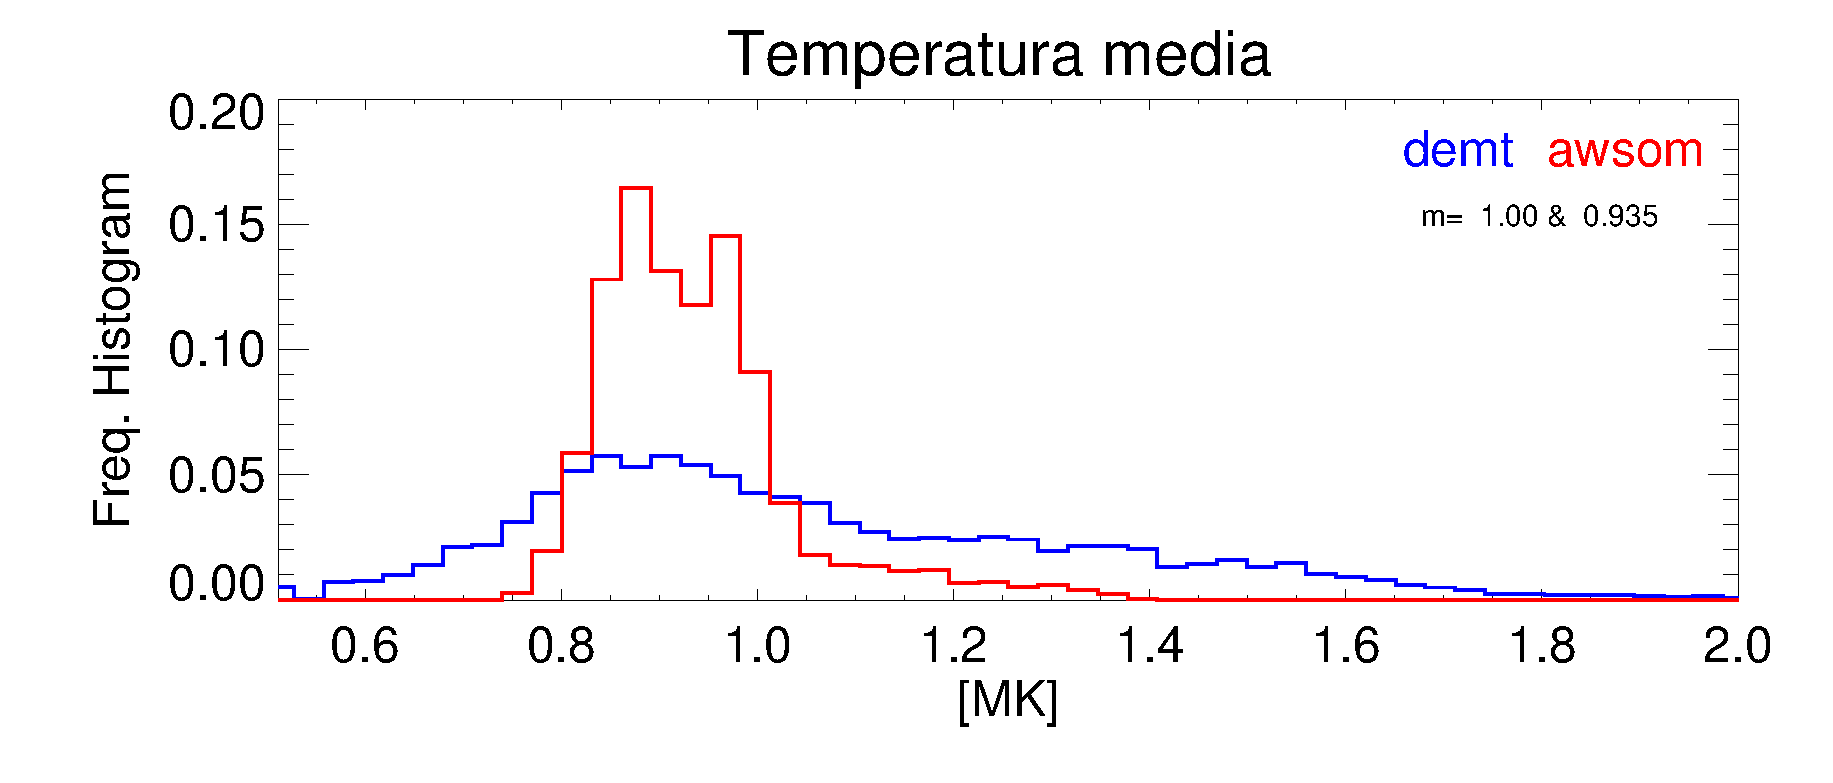
\includegraphics[width=0.32\textwidth]{figuras/proceeding_2208_demt_awsom_CH_Tm.eps}
  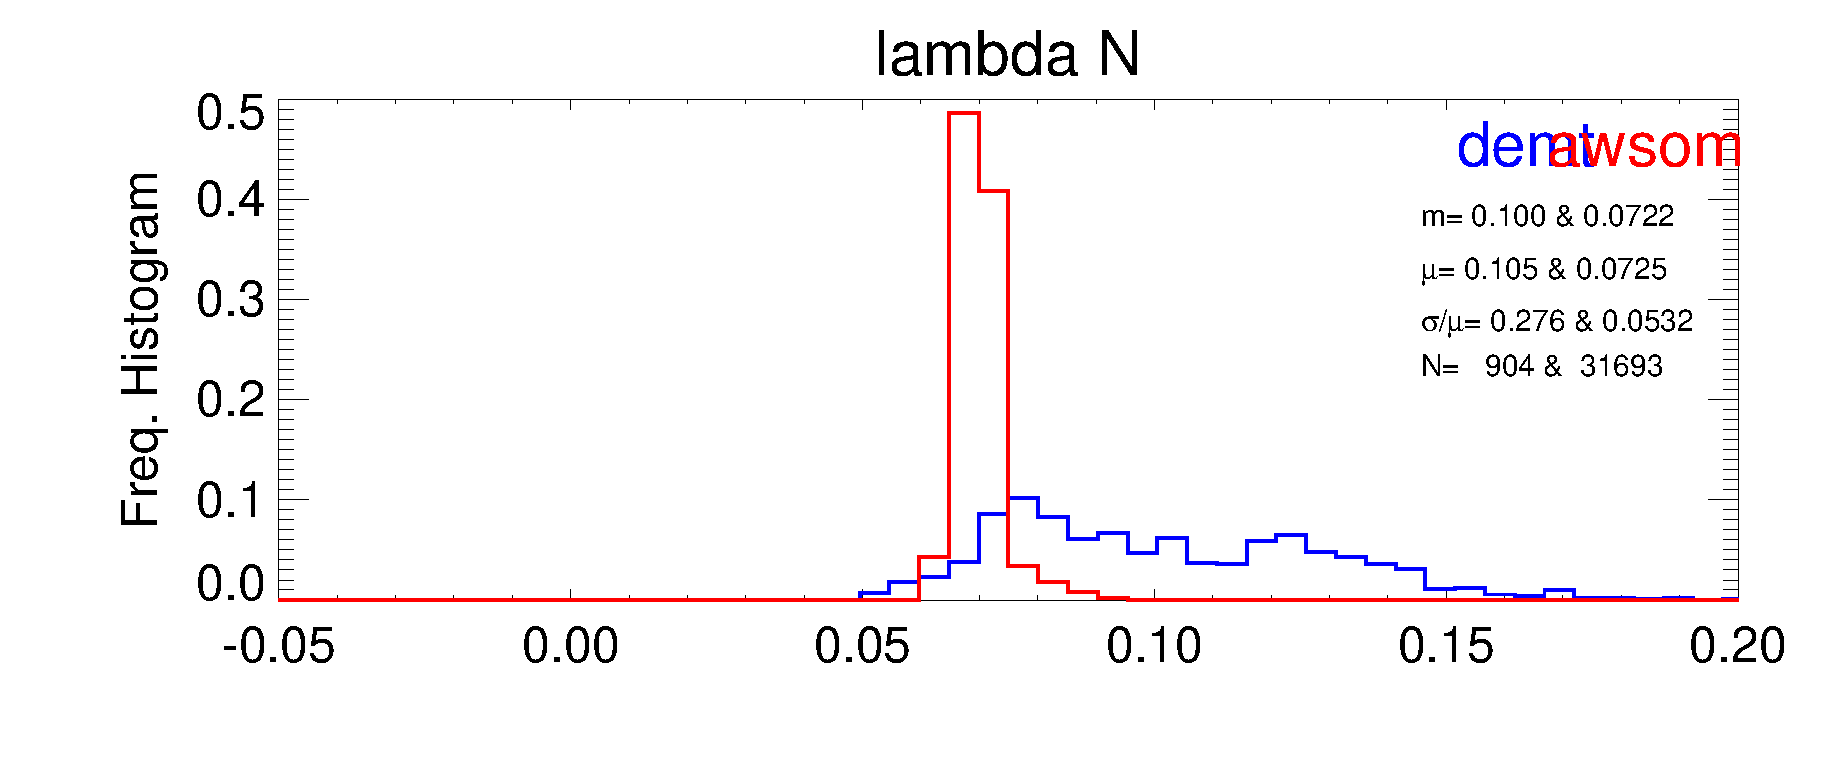
\includegraphics[width=0.32\textwidth]{figuras/proceeding_2208_demt_awsom_CH_lambda_n.eps}
  \caption{Histogramas}
  \label{fig-histos2}
\end{figure*}

\begin{acknowledgement}
\texttt{A Juan roberto Macri}
\end{acknowledgement}

%%%%%%%%%%%%%%%%%%%%%%%%%%%%%%%%%%%%%%%%%%%%%%%%%%%%%%%%%%%%%%%%%%%%%%%%%%%%%%
%                                                                            %
%  Por favor no modifique las líneas de la bibliografía, salvo el nombre     %
%  el archivo de Bibtex con la lista de citas (sin la extensión .BIB)        %
%                                                                            %
%  Please do not modify the following lines, except the name of the Bibtex   %
%  file (whithout the .BIB extension)                                        %
%                                                                            %
%%%%%%%%%%%%%%%%%%%%%%%%%%%%%%%%%%%%%%%%%%%%%%%%%%%%%%%%%%%%%%%%%%%%%%%%%%%%%% 

\bibliographystyle{baaa}
\small
\bibliography{bibliografia}
 
\end{document}
